
\documentclass[a4paper,11pt]{article}
\usepackage{geometry}
\geometry{margin=2cm}
\usepackage{booktabs}
\usepackage{graphicx}
\usepackage{amsmath}
\usepackage{siunitx}
\usepackage{caption}
\usepackage{times}
\usepackage[utf8]{inputenc}
\usepackage{tocloft}

\title{Spectral Simulation Report}
\author{Automated Analysis}
\date{\today}

\begin{document}

\maketitle
\tableofcontents
\clearpage

\section{Introduction}
This report presents the results of spectral simulations derived from HDF5 dataset analysis. Each sample includes a spectral plot and a detailed table summarizing the initial composition and actual labeled positions of elements, along with simulation parameters such as temperature and electron density.


\section{Sample: 19088}
\subsection{Simulation Parameters}
\begin{table}[h!]
    \centering
    \begin{tabular}{ll}
        \toprule
        \textbf{Parameter} & \textbf{Value} \\
        \midrule
        Temperature ($T$) & 9141 \,\si{K} \\
        Electron Density ($n_e$) & 2.31e+14 \,\si{cm^-3} \\
        \bottomrule
    \end{tabular}
    \caption{Simulation parameters for sample 19088.}
    \label{tab:params_19088}
\end{table}

\subsection{Composition Analysis}
\begin{table}[h!]
    \centering
    \begin{tabular}{lcc}
        \toprule
        \textbf{Element} & \textbf{Initial Composition (\%)} & \textbf{Actual Labeled Position (\%)} \\
        \midrule
        Al & 0.00 & 0.00 \\
        Ar & 0.00 & 0.00 \\
        C & 4.20 & 6.10 \\
        Ca & 15.34 & 3.66 \\
        Cl & 2.38 & 0.81 \\
        Co & 12.34 & 34.28 \\
        Cr & 3.73 & 9.69 \\
        Fe & 12.86 & 67.14 \\
        Mg & 8.78 & 8.35 \\
        Mn & 4.86 & 17.24 \\
        N & 7.36 & 9.79 \\
        Na & 9.64 & 7.86 \\
        Ni & 4.18 & 11.57 \\
        O & 0.00 & 0.00 \\
        S & 1.74 & 4.86 \\
        Si & 12.56 & 5.44 \\
        Ti & 0.00 & 0.00 \\
        background & N/A & 14.48 \\

        \midrule
        \textbf{Total (\%)} & & 201.27 \\
        \bottomrule
    \end{tabular}
    \caption{Composition analysis for sample 19088.}
    \label{tab:comp_19088}
\end{table}

\subsection{Spectral Plot}
\begin{figure}[h!]
    \centering
    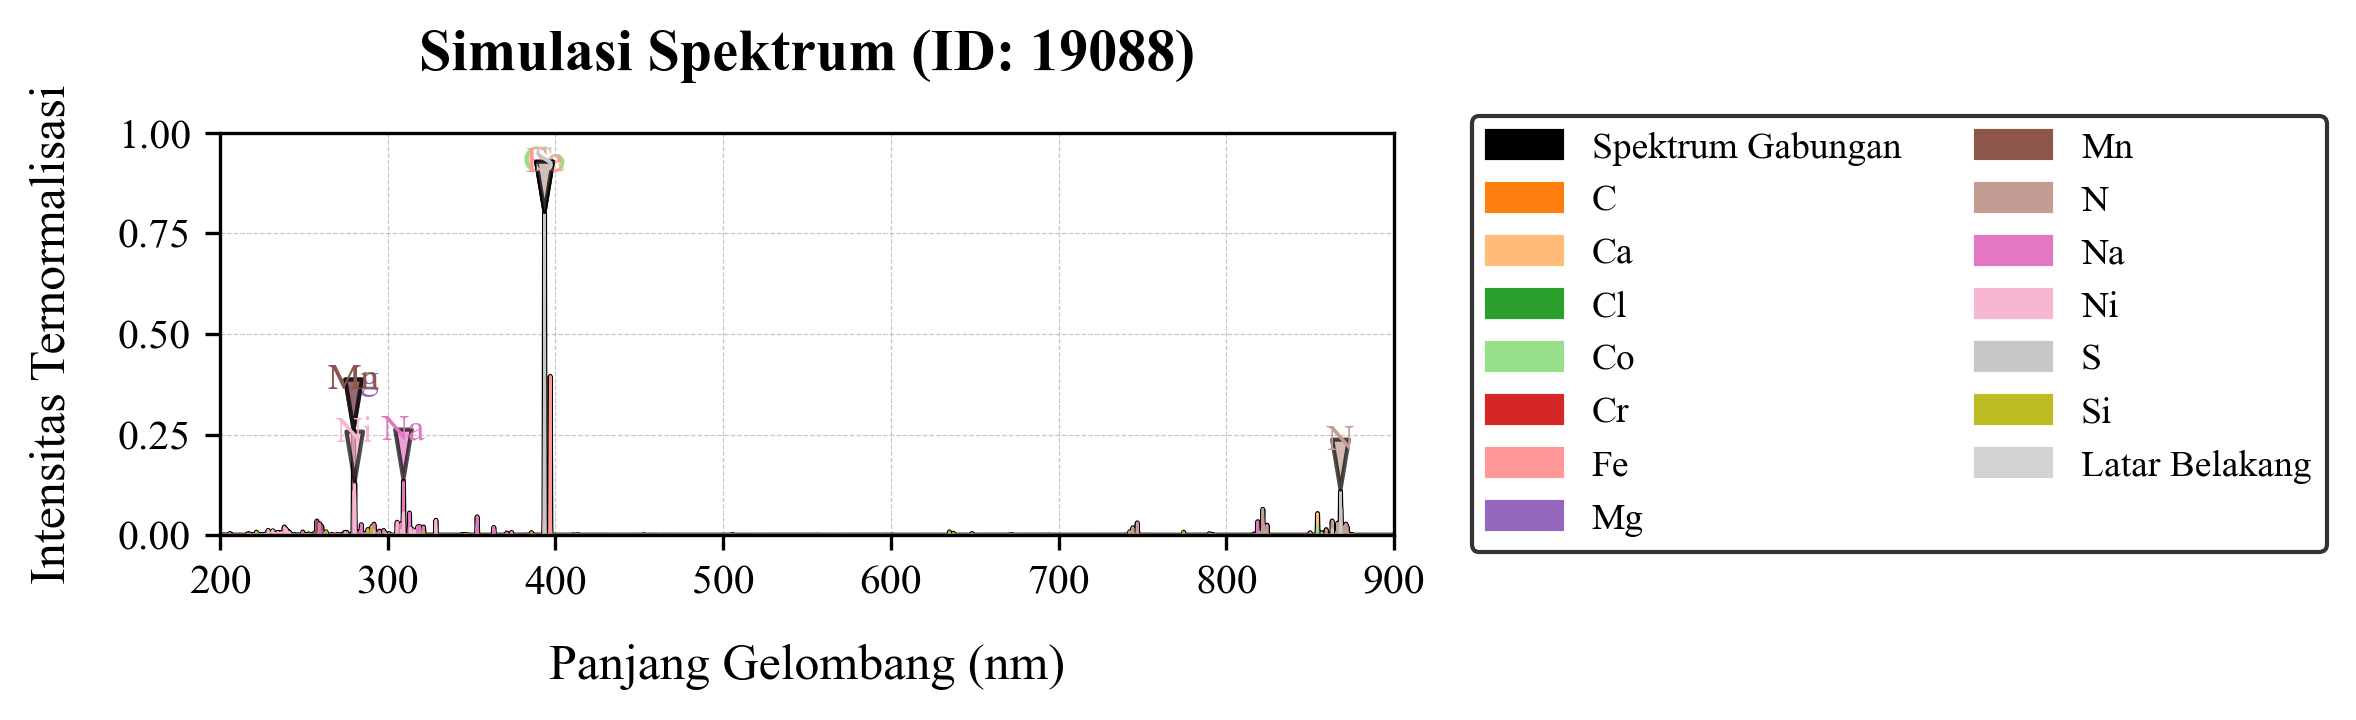
\includegraphics[width=0.9\textwidth]{spectrum_19088.png}
    \caption{Spectral simulation plot for sample 19088.}
    \label{fig:spectrum_19088}
\end{figure}

\clearpage

\section{Sample: 16764}
\subsection{Simulation Parameters}
\begin{table}[h!]
    \centering
    \begin{tabular}{ll}
        \toprule
        \textbf{Parameter} & \textbf{Value} \\
        \midrule
        Temperature ($T$) & 13081 \,\si{K} \\
        Electron Density ($n_e$) & 3.13e+15 \,\si{cm^-3} \\
        \bottomrule
    \end{tabular}
    \caption{Simulation parameters for sample 16764.}
    \label{tab:params_16764}
\end{table}

\subsection{Composition Analysis}
\begin{table}[h!]
    \centering
    \begin{tabular}{lcc}
        \toprule
        \textbf{Element} & \textbf{Initial Composition (\%)} & \textbf{Actual Labeled Position (\%)} \\
        \midrule
        Al & 10.62 & 11.28 \\
        Ar & 6.31 & 17.75 \\
        C & 7.26 & 17.90 \\
        Ca & 8.19 & 3.66 \\
        Cl & 8.37 & 0.85 \\
        Co & 7.27 & 34.28 \\
        Cr & 11.28 & 9.69 \\
        Fe & 0.00 & 0.00 \\
        Mg & 8.27 & 8.59 \\
        Mn & 9.04 & 17.24 \\
        N & 1.32 & 14.70 \\
        Na & 2.78 & 7.86 \\
        Ni & 1.59 & 11.55 \\
        O & 4.57 & 7.74 \\
        S & 8.48 & 5.52 \\
        Si & 4.66 & 5.44 \\
        Ti & 0.00 & 0.00 \\
        background & N/A & 18.04 \\

        \midrule
        \textbf{Total (\%)} & & 192.09 \\
        \bottomrule
    \end{tabular}
    \caption{Composition analysis for sample 16764.}
    \label{tab:comp_16764}
\end{table}

\subsection{Spectral Plot}
\begin{figure}[h!]
    \centering
    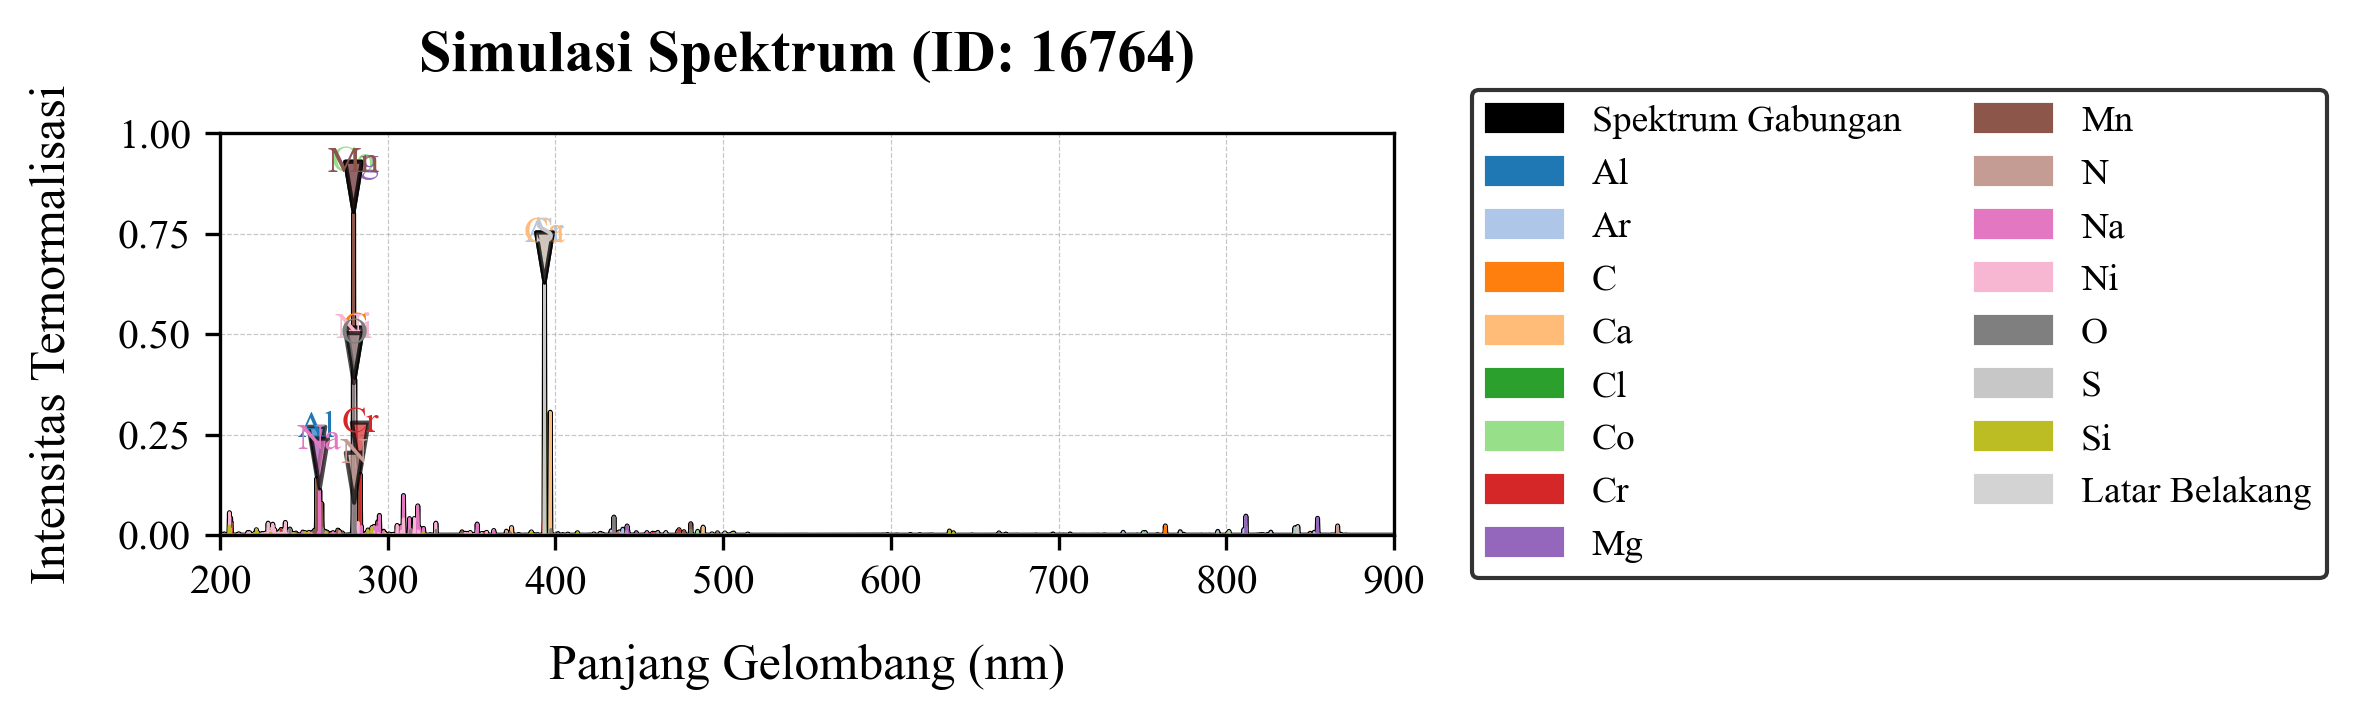
\includegraphics[width=0.9\textwidth]{spectrum_16764.png}
    \caption{Spectral simulation plot for sample 16764.}
    \label{fig:spectrum_16764}
\end{figure}

\clearpage

\section{Sample: 3467}
\subsection{Simulation Parameters}
\begin{table}[h!]
    \centering
    \begin{tabular}{ll}
        \toprule
        \textbf{Parameter} & \textbf{Value} \\
        \midrule
        Temperature ($T$) & 9242 \,\si{K} \\
        Electron Density ($n_e$) & 3.68e+14 \,\si{cm^-3} \\
        \bottomrule
    \end{tabular}
    \caption{Simulation parameters for sample 3467.}
    \label{tab:params_3467}
\end{table}

\subsection{Composition Analysis}
\begin{table}[h!]
    \centering
    \begin{tabular}{lcc}
        \toprule
        \textbf{Element} & \textbf{Initial Composition (\%)} & \textbf{Actual Labeled Position (\%)} \\
        \midrule
        Al & 5.21 & 10.72 \\
        Ar & 0.00 & 0.00 \\
        C & 0.00 & 0.00 \\
        Ca & 18.30 & 3.66 \\
        Cl & 10.98 & 0.85 \\
        Co & 0.00 & 0.00 \\
        Cr & 6.79 & 9.69 \\
        Fe & 0.00 & 0.00 \\
        Mg & 11.51 & 8.45 \\
        Mn & 5.42 & 17.24 \\
        N & 0.00 & 0.00 \\
        Na & 13.93 & 7.86 \\
        Ni & 4.20 & 11.62 \\
        O & 10.29 & 4.15 \\
        S & 8.89 & 5.40 \\
        Si & 4.49 & 5.40 \\
        Ti & 0.00 & 0.00 \\
        background & N/A & 44.24 \\

        \midrule
        \textbf{Total (\%)} & & 129.27 \\
        \bottomrule
    \end{tabular}
    \caption{Composition analysis for sample 3467.}
    \label{tab:comp_3467}
\end{table}

\subsection{Spectral Plot}
\begin{figure}[h!]
    \centering
    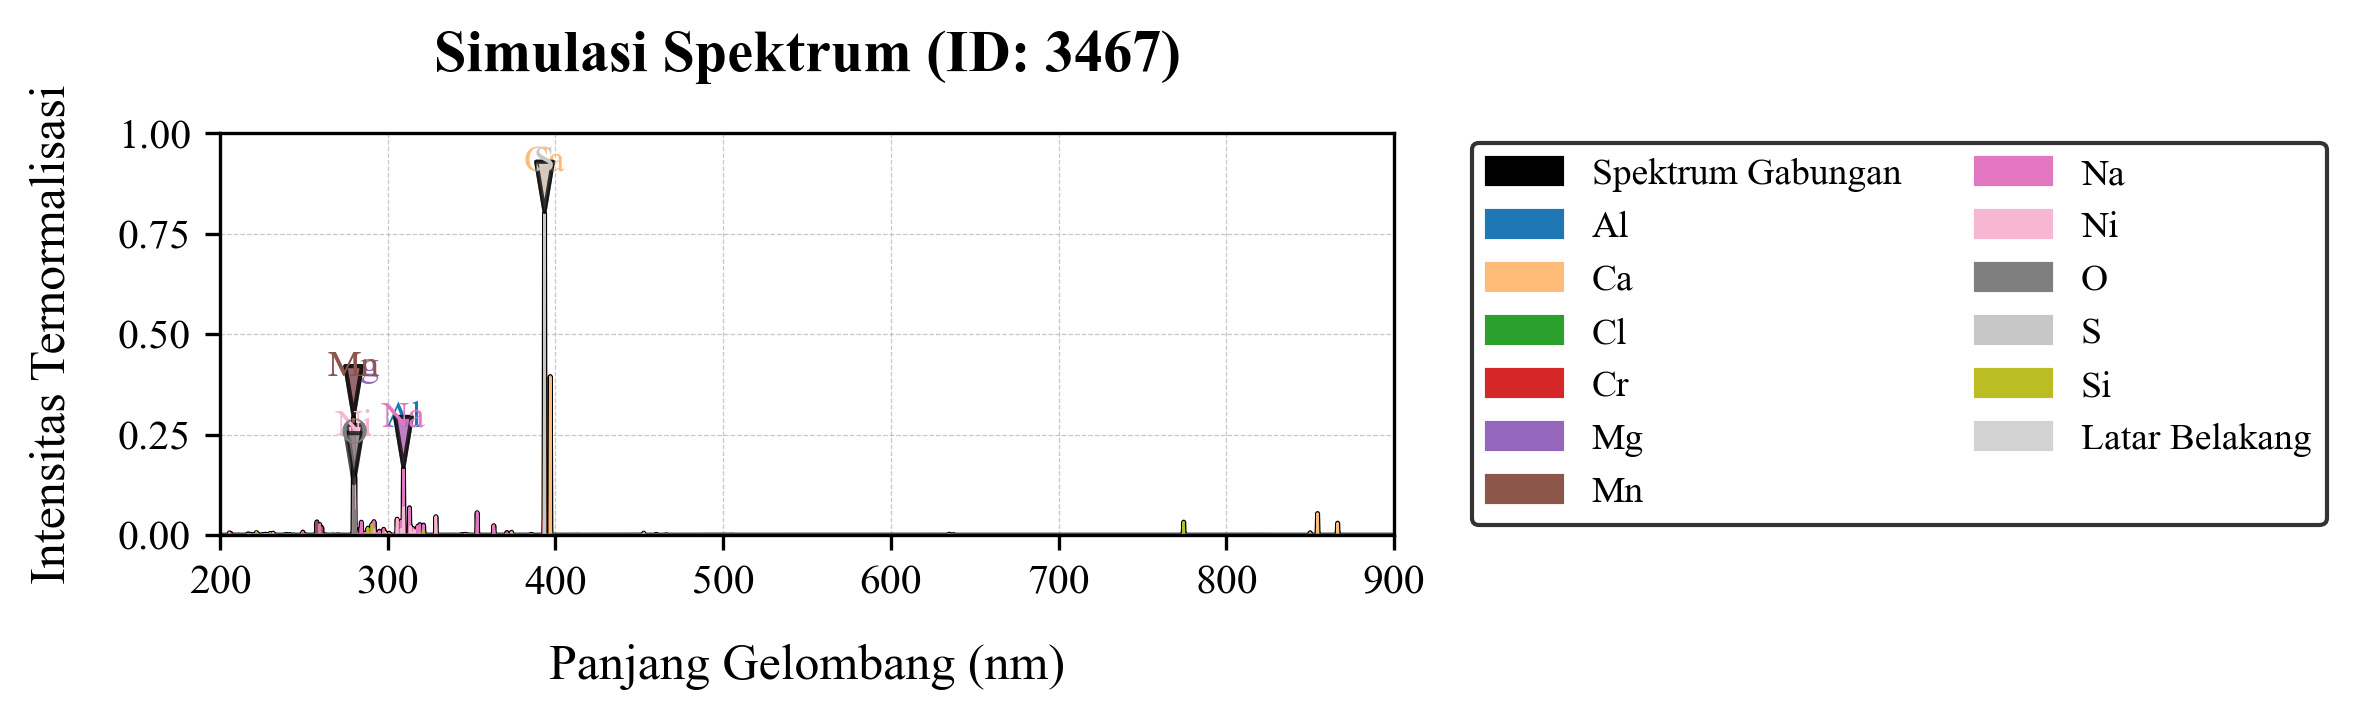
\includegraphics[width=0.9\textwidth]{spectrum_3467.png}
    \caption{Spectral simulation plot for sample 3467.}
    \label{fig:spectrum_3467}
\end{figure}

\clearpage

\section{Sample: 6423}
\subsection{Simulation Parameters}
\begin{table}[h!]
    \centering
    \begin{tabular}{ll}
        \toprule
        \textbf{Parameter} & \textbf{Value} \\
        \midrule
        Temperature ($T$) & 11162 \,\si{K} \\
        Electron Density ($n_e$) & 1.02e+15 \,\si{cm^-3} \\
        \bottomrule
    \end{tabular}
    \caption{Simulation parameters for sample 6423.}
    \label{tab:params_6423}
\end{table}

\subsection{Composition Analysis}
\begin{table}[h!]
    \centering
    \begin{tabular}{lcc}
        \toprule
        \textbf{Element} & \textbf{Initial Composition (\%)} & \textbf{Actual Labeled Position (\%)} \\
        \midrule
        Al & 0.00 & 0.00 \\
        Ar & 0.00 & 0.00 \\
        C & 0.00 & 0.00 \\
        Ca & 5.87 & 3.66 \\
        Cl & 8.92 & 0.85 \\
        Co & 8.05 & 34.28 \\
        Cr & 3.59 & 9.69 \\
        Fe & 10.25 & 67.33 \\
        Mg & 11.99 & 8.59 \\
        Mn & 15.41 & 17.24 \\
        N & 0.00 & 0.00 \\
        Na & 7.24 & 7.86 \\
        Ni & 4.60 & 11.57 \\
        O & 0.00 & 0.00 \\
        S & 7.84 & 5.57 \\
        Si & 16.24 & 5.44 \\
        Ti & 0.00 & 0.00 \\
        background & N/A & 17.92 \\

        \midrule
        \textbf{Total (\%)} & & 190.01 \\
        \bottomrule
    \end{tabular}
    \caption{Composition analysis for sample 6423.}
    \label{tab:comp_6423}
\end{table}

\subsection{Spectral Plot}
\begin{figure}[h!]
    \centering
    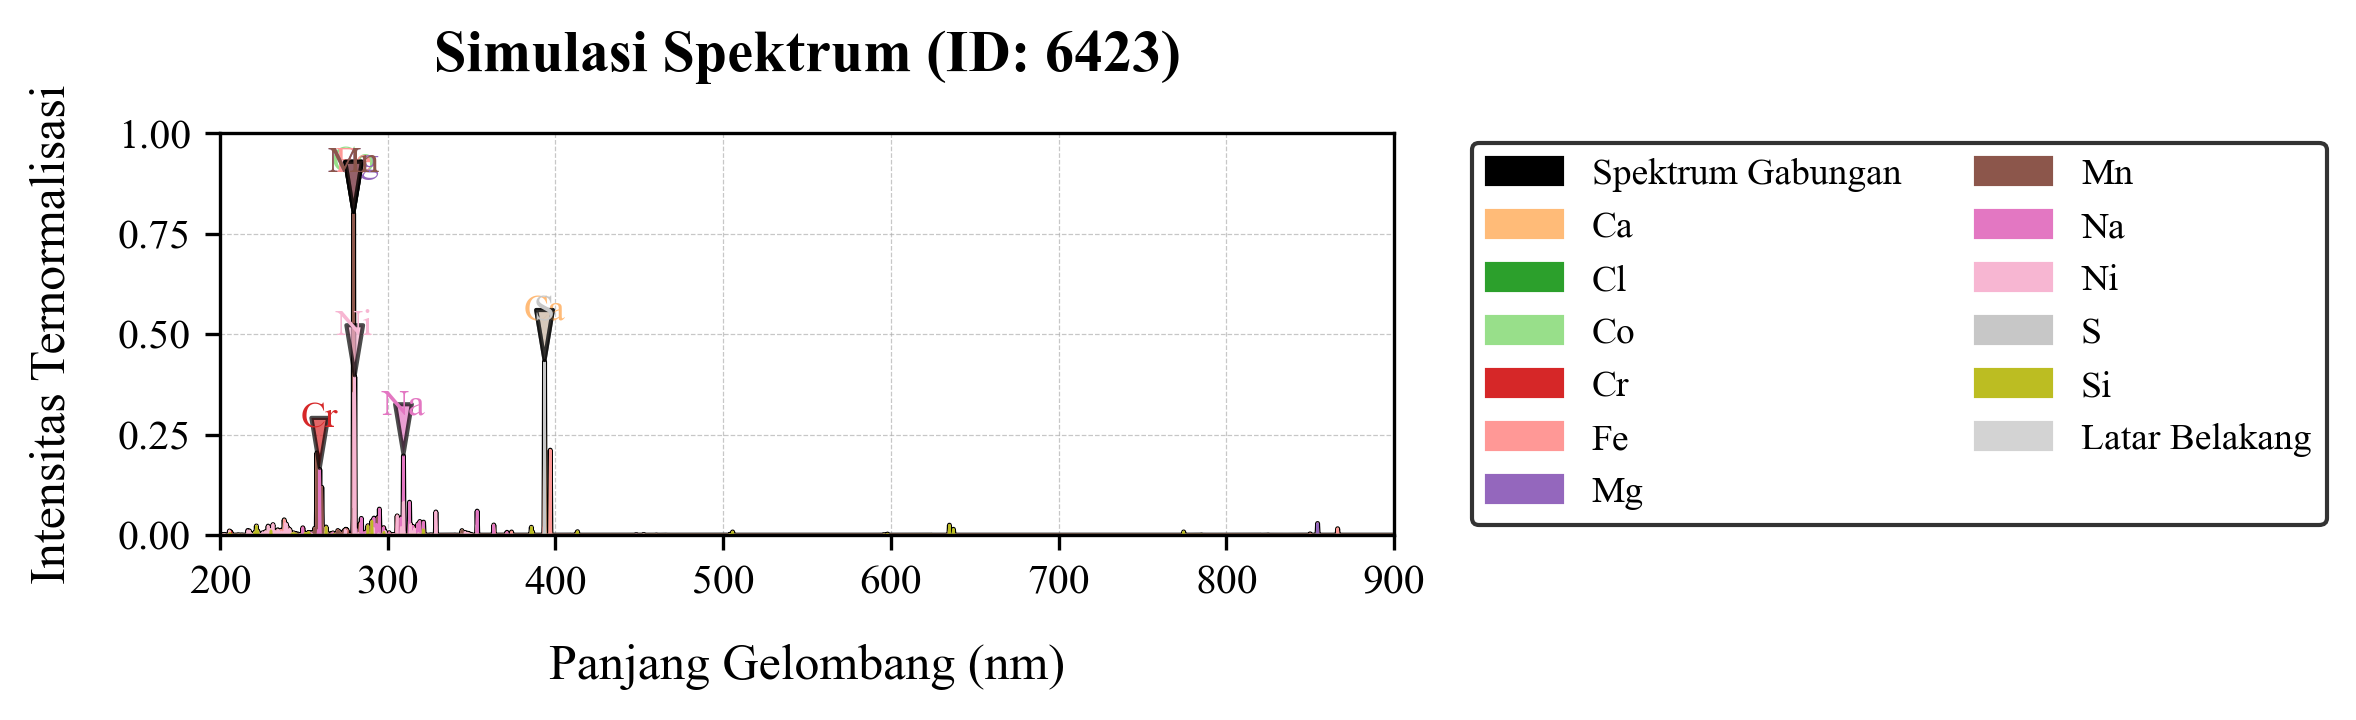
\includegraphics[width=0.9\textwidth]{spectrum_6423.png}
    \caption{Spectral simulation plot for sample 6423.}
    \label{fig:spectrum_6423}
\end{figure}

\clearpage

\section{Sample: 13548}
\subsection{Simulation Parameters}
\begin{table}[h!]
    \centering
    \begin{tabular}{ll}
        \toprule
        \textbf{Parameter} & \textbf{Value} \\
        \midrule
        Temperature ($T$) & 12071 \,\si{K} \\
        Electron Density ($n_e$) & 3.35e+14 \,\si{cm^-3} \\
        \bottomrule
    \end{tabular}
    \caption{Simulation parameters for sample 13548.}
    \label{tab:params_13548}
\end{table}

\subsection{Composition Analysis}
\begin{table}[h!]
    \centering
    \begin{tabular}{lcc}
        \toprule
        \textbf{Element} & \textbf{Initial Composition (\%)} & \textbf{Actual Labeled Position (\%)} \\
        \midrule
        Al & 11.72 & 11.28 \\
        Ar & 0.00 & 0.00 \\
        C & 0.00 & 0.00 \\
        Ca & 17.72 & 3.66 \\
        Cl & 4.47 & 0.85 \\
        Co & 0.00 & 0.00 \\
        Cr & 8.59 & 9.69 \\
        Fe & 0.00 & 0.00 \\
        Mg & 16.48 & 8.54 \\
        Mn & 7.19 & 17.24 \\
        N & 0.00 & 0.00 \\
        Na & 0.92 & 7.69 \\
        Ni & 17.46 & 11.57 \\
        O & 0.00 & 0.00 \\
        S & 14.71 & 5.52 \\
        Si & 0.74 & 5.30 \\
        Ti & 0.00 & 0.00 \\
        background & N/A & 45.31 \\

        \midrule
        \textbf{Total (\%)} & & 126.66 \\
        \bottomrule
    \end{tabular}
    \caption{Composition analysis for sample 13548.}
    \label{tab:comp_13548}
\end{table}

\subsection{Spectral Plot}
\begin{figure}[h!]
    \centering
    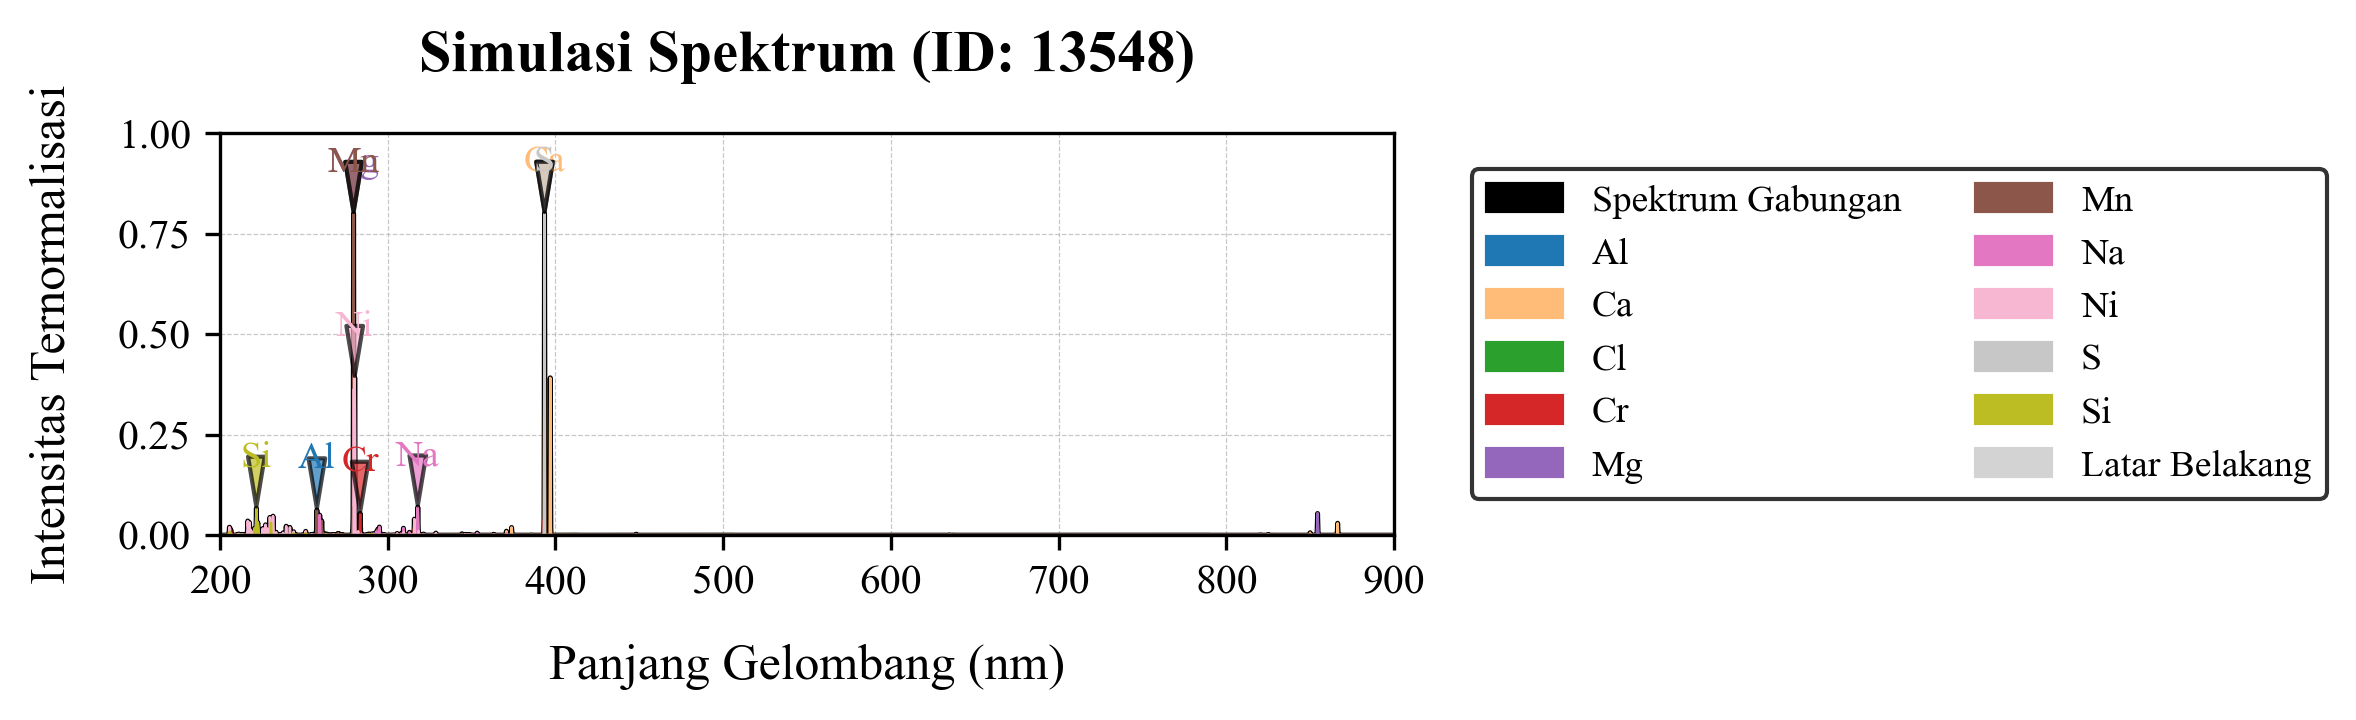
\includegraphics[width=0.9\textwidth]{spectrum_13548.png}
    \caption{Spectral simulation plot for sample 13548.}
    \label{fig:spectrum_13548}
\end{figure}

\clearpage

\end{document}
